\documentclass[11pt,a4paper]{article}

\usepackage[margin=1in]{geometry}
\usepackage{graphicx}
\usepackage{float}
\usepackage{amsmath}
\usepackage{titlesec}
\usepackage{parskip}
\usepackage{hyperref}
\usepackage{fancyhdr}
\usepackage{xcolor}

\pagestyle{fancy}
\fancyhf{}
\rhead{Computer Architecture Lab T2}
\lhead{RISC-V Processor Report}
\rfoot{Page \thepage}

\titleformat{\section}{\large\bfseries}{}{0em}{}

\begin{document}

\begin{center}
{\LARGE \textbf{Course Project Report}}\\[0.3em]
\textbf{RISC-V Processor Implementation}\\[1em]

\textbf{Areesha Kashif, Alishbah Saleem Kath, Sarah Fatima}\\
\textbf{Instructor: Ms. Maham Tabassum}
\end{center}

% ==========================================================
\section{Processor Summary and Synthesis:}

The implemented processor is a single-cycle RV32I design where all stages
(fetch, decode, execute, memory, write-back) complete in one clock cycle.

The datapath consists of:
\begin{itemize}
\item Program Counter (PC) for instruction sequencing
\item Instruction Memory (read-only)
\item Register File (32 registers, 2 read and 1 write)
\item ALU for arithmetic and logical operations
\item Immediate Generator for instruction formats
\item Data Memory for load/store operations
\item Control Unit (main and ALU control)
\end{itemize}

Multiplexers control data flow between ALU inputs, write back source,
and next PC selection.

\textbf{Synthesis:}
The design was written in Verilog and implemented on the Basys 3 FPGA.
The standard flow was used:
\begin{itemize}
\item Functional Simulation
\item Synthesis and Implementation
\item Bitstream Generation
\end{itemize}

A clock divider was used to slow execution for observation.

\subsection*{Task A: Countdown Program Implementation}

Task A implements a control-flow program that performs input reading, countdown execution, and continuous looping using jump instructions.

\subsubsection*{Program Behavior}

The program reads an input value from a fixed memory-mapped address and displays it on the seven-segment display. Execution is then transferred to a countdown routine using a \texttt{jal} instruction, which stores the return address in \texttt{ra}.

Inside the countdown loop, the value is decremented using the ALU and continuously checked using a branch instruction. After completion, control returns to the main program, forming a continuous execution cycle.

\subsubsection*{Processor Features Used:} 
\begin{itemize}
\item The countdown routine is executed using a \texttt{jal} instruction, which stores the return address in \texttt{ra} and transfers control to the function.

\item Inside the countdown loop, the value is decremented using the ALU and repeatedly checked using branch instructions.

\item The stack is used to preserve the return address and temporary registers during function calls, ensuring correct program execution flow.

\item Conditional branching is used to control loop continuation and termination, while reset behavior demonstrates external control flow through the FPGA reset signal.

\item After completing the countdown, the program returns to the input stage using an unconditional jump, forming a continuous execution cycle.
\end{itemize}
\begin{figure}[H]
\centering
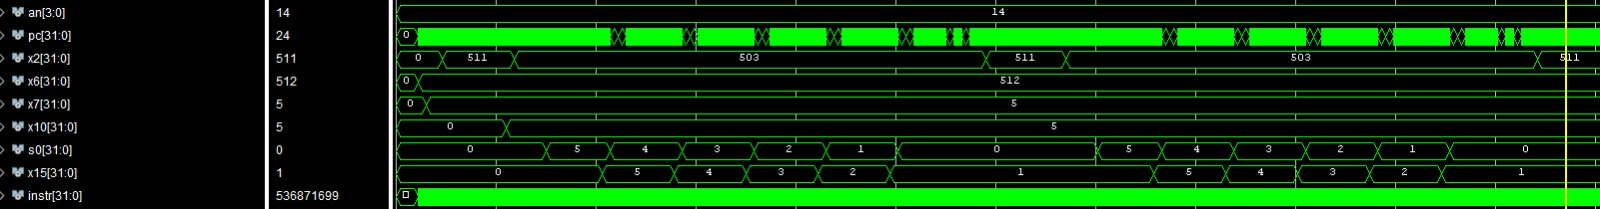
\includegraphics[width=1.1\textwidth]{taskA.png}
\caption{Task A Simulation}
\end{figure}

% ==========================================================
\section{Task B: New Instructions}

Three new instructions were added: SLTI, SRA, and BLTU.

\subsection{SLTI (Set Less Than Immediate)}

\textbf{Operation:} rd = (rs1 < imm)

Implemented by extending ALU control for funct3 = 010 under I-type.
The ALU performs signed comparison and outputs 1 or 0.

\subsection{SRA (Shift Right Arithmetic)}

\textbf{Operation:} rd = rs1 \texttt{>>>} rs2

Implemented by distinguishing funct7 bit in ALU control.
ALU uses signed shift to preserve sign bits.

\subsection{BLTU (Branch if Less Than Unsigned)}

\textbf{Operation:} branch if rs1 < rs2 (unsigned)

Implemented by:
\begin{itemize}
\item Adding unsigned comparison in ALU
\item Extending branch logic to include funct3 = 110
\end{itemize}

% ==========================================================
% EXTRA PART B ADDITION (DO NOT REMOVE EXISTING CONTENT)
% ==========================================================
\subsection*{Table: Main Control Unit}

\begin{table}[H]
\centering
\resizebox{\textwidth}{!}{
\begin{tabular}{lccccccccc}
\hline
Instruction & Type & Opcode & RegWrite & ALUSrc & MemRead & MemWrite & MemtoReg & Branch & ALUOp \\
\hline
SLTI  & I & 0010011 & 1 & 1 & 0 & 0 & 0 & 0 & 11 \\
SRA   & R & 0110011 & 1 & 0 & 0 & 0 & 0 & 0 & 10 \\
BLTU  & B & 1100011 & 0 & 0 & 0 & 0 & 0 & 1 & 01 \\
\hline
\end{tabular}
}
\end{table}

\subsection*{Table: ALU Control Unit}

\begin{table}[H]
\centering
\begin{tabular}{lccccc}
\hline
Instruction & ALUOp & funct3 & funct7[5] & ALUControl & Operation \\
\hline
SLTI  & 11 & 010 & X & 0111 & Signed Less Than \\
SRA   & 10 & 101 & 1 & 1000 & Shift Right Arithmetic \\
BLTU  & 01 & 110 & X & 1001 & Unsigned Less Than \\
\hline
\end{tabular}
\end{table}

\subsection*{Execution / LED Verification}

\begin{table}[H]
\centering
\begin{tabular}{ccc}
\hline
PC (7-seg) & Instruction & LED Pattern [15:4] \\
\hline
12  & SLTI & 1100 0011 0111 \\
16  & SLTI & 1100 0011 0111 \\
20  & SRA  & 1000 0010 1000 \\
28  & SRA  & 1000 0010 1000 \\
40  & BLTU & 0000 0101 1001 \\
48  & BLTU taken & 0000 0101 1101 \\
\hline
\end{tabular}
\end{table}

\begin{figure}[H]
\centering
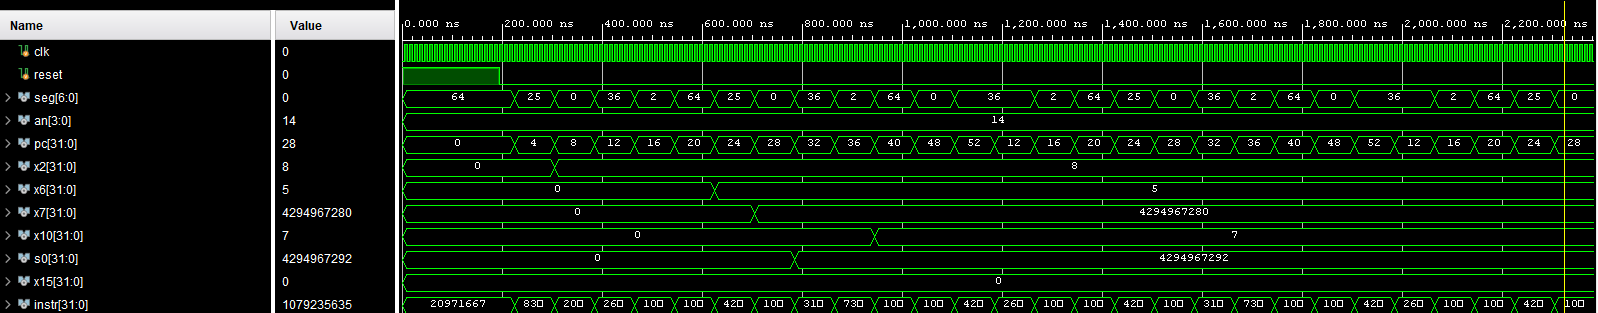
\includegraphics[width=1.1\textwidth]{taskB.png}
\caption{Task B Simulation}
\end{figure}

% ==========================================================
\section{Task C: GCD (Greatest Common Divisor) Program Description}

A GCD calculator was implemented using the subtraction-based Euclidean algorithm.

\textbf{Functionality:}
\begin{itemize}
\item Inputs taken from memory-mapped addresses (0x200, 0x204)
\item Start signal from 0x20C
\item Output written to 0x208 (7-segment display)
\end{itemize}

\textbf{Algorithm:}
\begin{itemize}
\item If $a > b$, subtract $b$ from $a$
\item If $b > a$, subtract $a$ from $b$
\item Repeat until $a = b$
\end{itemize}

\textbf{Implementation Details:}
\begin{itemize}
\item Uses a subroutine with proper stack handling
\item Return address (ra) is saved and restored using stack
\item Loop uses conditional branching (including BLTU)
\end{itemize}

\subsection{FSM Representation}

\begin{figure}[H]
\centering

\begin{minipage}{0.5\textwidth}
\centering
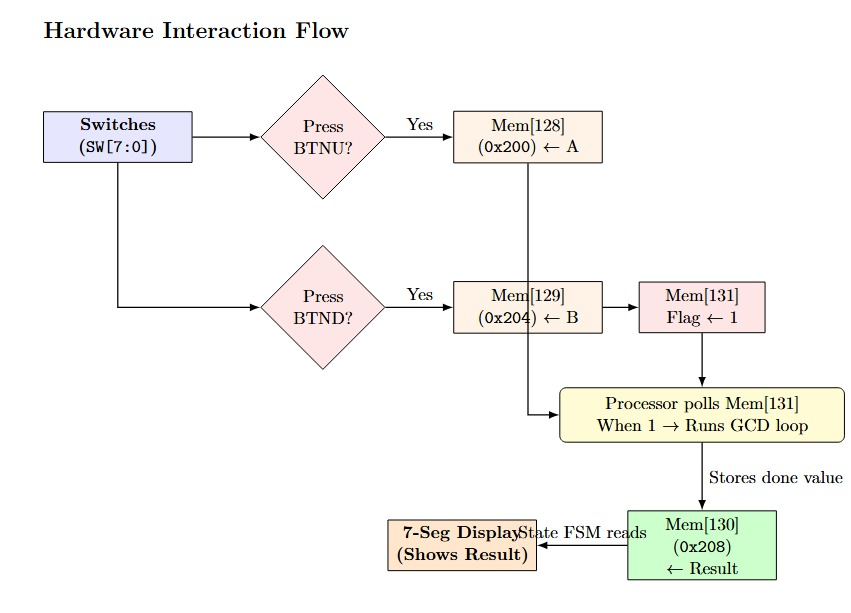
\includegraphics[width=\textwidth]{flow.png}
\end{minipage}
\hfill
\begin{minipage}{0.5\textwidth}
\centering
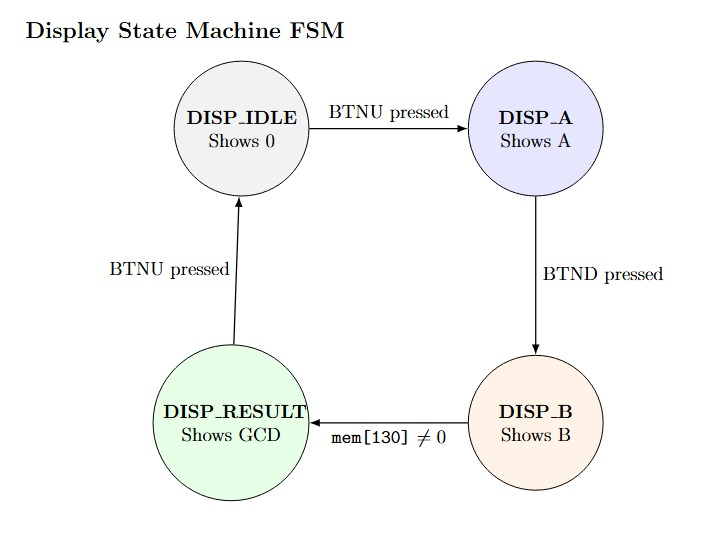
\includegraphics[width=\textwidth]{fsm.png}
\end{minipage}

\caption{Task C FSM Diagrams}
\end{figure}

\subsection{Simulation}

\begin{figure}[H]
\centering
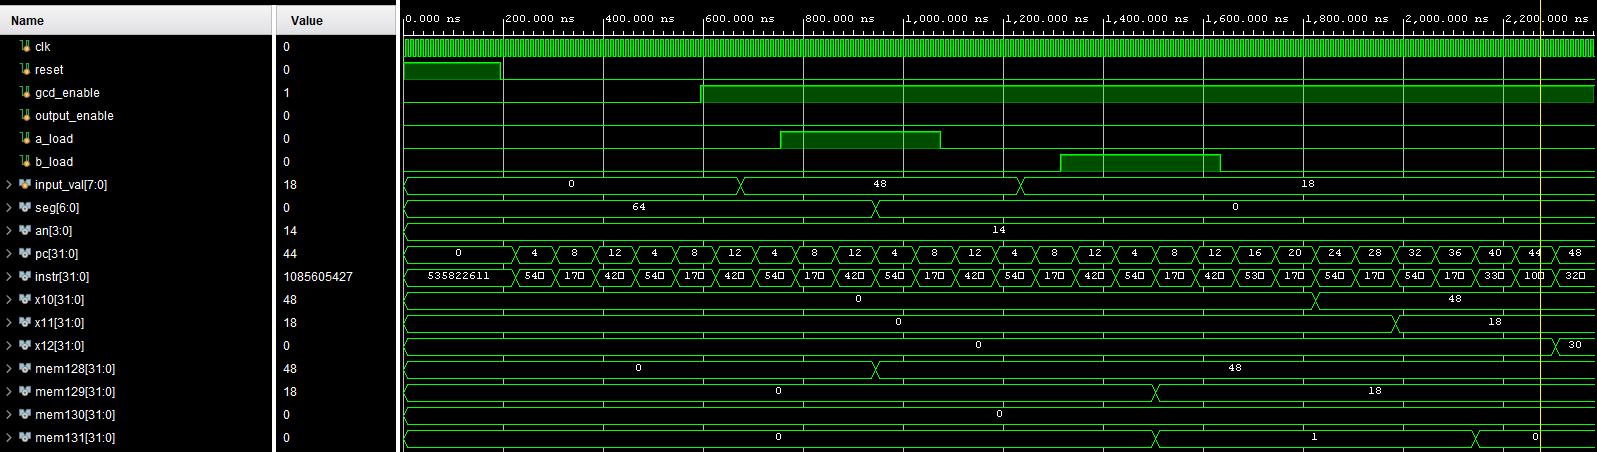
\includegraphics[width=1.1\textwidth]{taskC.png}
\caption{Task C Simulation}
\end{figure}
% ==========================================================
\subsection*{Source Code:}
GitHub Repository: \url{https://github.com/Areesha06/CALabs-Git-AreeshaKashif/tree/main/Project}

\end{document}